\documentclass{fkpresentation}

% Information to be included in the title page:
\title{\textmd{Seeing is Believing}}
\author{Forest Kobayashi}
\institute{Harvey Mudd College}
\date{February 18th, 2018}


\usetheme{Dresden}
\usecolortheme{crane}
% Partial differential
\newcommand{\pdd}{\mathop{}\,\partial}

% Total differential
\newcommand{\dd}{\mathop{}\,\mathrm{d}}

% Define partial derivative and ordinary derivative things
\newcommand{\pd}[3][]{\frac{\partial^{#1}\hspace{-.08em} {#2}}{\partial {#3}^{#1}}}
\newcommand{\od}[3][]{\frac{{d}^{#1}\hspace{-.08em} {#2}}{d {#3}^{#1}}}

\usetikzlibrary{quotes,arrows.meta}
\tikzset{
  annotated cuboid/.pic={
    \tikzset{%
      every edge quotes/.append style={midway, auto},
      /cuboid/.cd,
      #1
    }
    \draw [every edge/.append style={pic actions, densely dashed, opacity=.5}, pic actions]
    (0,0,0) coordinate (o) -- ++(-\cubescale*\cubex,0,0) coordinate (a) -- ++(0,-\cubescale*\cubey,0) coordinate (b) edge coordinate [pos=1] (g) ++(0,0,-\cubescale*\cubez)  -- ++(\cubescale*\cubex,0,0) coordinate (c) -- cycle
    (o) -- ++(0,0,-\cubescale*\cubez) coordinate (d) -- ++(0,-\cubescale*\cubey,0) coordinate (e) edge (g) -- (c) -- cycle
    (o) -- (a) -- ++(0,0,-\cubescale*\cubez) coordinate (f) edge (g) -- (d) -- cycle;
    \path [every edge/.append style={pic actions, |-|}]
    (b) +(0,-5pt) coordinate (b1) edge ["\cubex \cubeunits"'] (b1 -| c)
    (b) +(-5pt,0) coordinate (b2) edge ["\cubey \cubeunits"] (b2 |- a)
    (c) +(3.5pt,-3.5pt) coordinate (c2) edge ["\cubez \cubeunits"'] ([xshift=3.5pt,yshift=-3.5pt]e)
    ;
  },
  /cuboid/.search also={/tikz},
  /cuboid/.cd,
  width/.store in=\cubex,
  height/.store in=\cubey,
  depth/.store in=\cubez,
  units/.store in=\cubeunits,
  scale/.store in=\cubescale,
  width=10,
  height=10,
  depth=10,
  units=cm,
  scale=.1,
}

\usepackage[style=british]{csquotes}

\def\signed #1{{\leavevmode\unskip\nobreak\hfil\penalty50\hskip1em
    \hbox{}\nobreak\hfill #1%
    \parfillskip=0pt \finalhyphendemerits=0 \endgraf}}

\newsavebox\mybox
\newenvironment{aquote}[1]
{\savebox\mybox{#1}\begin{quote}\openautoquote\hspace*{-.7ex}}
  {\unskip\closeautoquote\vspace*{1mm}\signed{\usebox\mybox}\end{quote}}


\begin{document}
\frame{\titlepage}
\section{Introduction}

\begin{frame}{A sum identity}{}
  \begin{theorem}
    Let $n \in \mathbb{N}$. Then
    \[\small
      \sum_{k=1}^n k = \frac{n(n+1)}{2}
    \]
  \end{theorem}\pause
  \begin{proof}
    Induct on $n$.
    \[\small
      \frac{k(k+1)}{2} + (k+1) = \frac{(k^2 + k) + (2k+2)}{2} = \frac{(k+1)(k+2)}{2}.
    \]
  \end{proof}
\end{frame}
\begin{frame}{The question}
  \vfill
  \begin{center}\large
    Why should you expect the formula to look like this?
  \end{center}
  \vfill
\end{frame}
\begin{frame}{Consternation }
  \begin{itemize}
    \item Bothered me a lot in high school
      \begin{itemize}
        \item Teachers: ``because the induction works''
        \item Eventually gave up on a deeper perspective
      \end{itemize}
    \item College
      \begin{itemize}
        \item Didn't question the inductive proof
      \end{itemize}
    \item Winter break
  \end{itemize}
\end{frame}
\begin{frame}{The challenge}
  \vfill
  \begin{aquote}{My Neighbor}
    I think that I just don't work well in abstraction. I care about the
    tangible, and things that I can \emph{see}.
  \end{aquote}
  \vfill
\end{frame}
\section{Warming up}
\begin{frame}{Desired explanation}
  \begin{itemize}
    \item Brief
    \item Accessible % to a non-technical audience, and
    \item Visualizable
  \end{itemize}
\end{frame}
\begin{frame}{Drawing a picture}{}
  Partial sums
  \begin{figure}[H]
    \flushleft
    \begin{tikzpicture}[scale=.95]
      \foreach \n in {0}{
        \pgfmathsetmacro{\sum}{.5*(\n*(\n+1))};
        \pgfmathsetmacro{\startx}{\sum+2*\n};
        \pgfmathsetmacro{\endx}{\startx+\n};
        \pgfmathsetmacro{\endy}{\n+1};
        \foreach \x in {0,...,\n}{
          \pgfmathsetmacro{\newx}{\x+\startx};
          \foreach \y in {0,1,...,\endy}{
            \pgfmathsetmacro{\labely}{\endy-\y};
            \pgfmathtruncatemacro{\whyyy}{round(\y+1)};
            \ifthenelse{\x=0}
            {\ifthenelse{\y=\endy}
              {}
              {\node at (\newx-.5,\labely-.5) {\whyyy}}}
            {}
            ;
            \pgfmathparse{(\x) < 0.001 ? int(1) : int(0)}
            \ifnum\pgfmathresult=1
            \pgfmathparse{(\y) > 1.001 ? int(1) : int(0)}
            \ifnum\pgfmathresult=1
            \node at (\newx-.5,\y-1) {$+$};
            \fi
            \fi
            \ifthenelse{\y=0}
            {\pgfmathparse{(\x + \y - \n) < 0.001 ? int(1) : int(0)}
              \ifnum\pgfmathresult=1
              \fill[fill=red, opacity=.4] (\newx,\y) rectangle (\newx+1,\y+1);
              \draw (\newx,\y) rectangle (\newx+1,\y+1);
              \fi}
            {\pgfmathparse{(\x + \y - \n) < 0.001 ? int(1) : int(0)}
              \ifnum\pgfmathresult=1
              \fill[fill=green, opacity=.4] (\newx,\y) rectangle (\newx+1,\y+1);
              \draw (\newx,\y) rectangle (\newx+1,\y+1);
              \fi}
          }
        }
        \pgfmathsetmacro{\nodex}{.5*(\startx+\endx+1)};
        \pgfmathtruncatemacro{\noden}{round(\n+1)};
        \pgfmathtruncatemacro{\nodesum}{round((\n+1)*(\n+2)*.5)};
        \node[anchor=north] at (\nodex, 0) {$S(\noden)$=\nodesum};
      }
    \end{tikzpicture}
  \end{figure}\pause
  \begin{figure}[H]
    \flushleft
    \begin{tikzpicture}[scale=.95]
      \foreach \n in {1}{
        \pgfmathsetmacro{\sum}{.5*(\n*(\n+1))};
        \pgfmathsetmacro{\startx}{\sum+2*\n};
        \pgfmathsetmacro{\endx}{\startx+\n};
        \pgfmathsetmacro{\endy}{\n+1};
        \foreach \x in {0,...,\n}{
          \pgfmathsetmacro{\newx}{\x+\startx};
          \foreach \y in {0,1,...,\endy}{
            \pgfmathsetmacro{\labely}{\endy-\y};
            \pgfmathtruncatemacro{\whyyy}{round(\y+1)};
            \ifthenelse{\x=0}
            {\ifthenelse{\y=\endy}
              {}
              {\node at (\newx-.5,\labely-.5) {\whyyy}}}
            {}
            ;
            \pgfmathparse{(\x) < 0.001 ? int(1) : int(0)}
            \ifnum\pgfmathresult=1
            \pgfmathparse{(\y) > 1.001 ? int(1) : int(0)}
            \ifnum\pgfmathresult=1
            \node at (\newx-.5,\y-1) {$+$};
            \fi
            \fi
            \ifthenelse{\y=0}
            {\pgfmathparse{(\x + \y - \n) < 0.001 ? int(1) : int(0)}
              \ifnum\pgfmathresult=1
              \fill[fill=red, opacity=.4] (\newx,\y) rectangle (\newx+1,\y+1);
              \draw (\newx,\y) rectangle (\newx+1,\y+1);
              \fi}
            {\pgfmathparse{(\x + \y - \n) < 0.001 ? int(1) : int(0)}
              \ifnum\pgfmathresult=1
              \fill[fill=green, opacity=.4] (\newx,\y) rectangle (\newx+1,\y+1);
              \draw (\newx,\y) rectangle (\newx+1,\y+1);
              \fi}
          }
        }
        \pgfmathsetmacro{\nodex}{.5*(\startx+\endx+1)};
        \pgfmathtruncatemacro{\noden}{round(\n+1)};
        \pgfmathtruncatemacro{\nodesum}{round((\n+1)*(\n+2)*.5)};
        \node[anchor=north] at (\nodex, 0) {$S(\noden)$=\nodesum};
      }
    \end{tikzpicture}
  \end{figure}
\end{frame}
\begin{frame}{Continuing}
  \begin{figure}[H]
    \centering
    \begin{tikzpicture}[scale=.67]
      \foreach \n in {2,3,4}{
        \pgfmathsetmacro{\sum}{.5*(\n*(\n+1))};
        \pgfmathsetmacro{\startx}{\sum+2*\n};
        \pgfmathsetmacro{\endx}{\startx+\n};
        \pgfmathsetmacro{\endy}{\n+1};
        \foreach \x in {0,...,\n}{
          \pgfmathsetmacro{\newx}{\x+\startx};
          \foreach \y in {0,1,...,\endy}{
            \pgfmathsetmacro{\labely}{\endy-\y};
            \pgfmathtruncatemacro{\whyyy}{round(\y+1)};
            \ifthenelse{\x=0}
            {\ifthenelse{\y=\endy}
              {}
              {\node at (\newx-.5,\labely-.5) {\whyyy}}}
            {}
            ;
            \pgfmathparse{(\x) < 0.001 ? int(1) : int(0)}
            \ifnum\pgfmathresult=1
            \pgfmathparse{(\y) > 1.001 ? int(1) : int(0)}
            \ifnum\pgfmathresult=1
            \node at (\newx-.5,\y-1) {$+$};
            \fi
            \fi
            \ifthenelse{\y=0}
            {\pgfmathparse{(\x + \y - \n) < 0.001 ? int(1) : int(0)}
              \ifnum\pgfmathresult=1
              \fill[fill=red, opacity=.4] (\newx,\y) rectangle (\newx+1,\y+1);
              \draw (\newx,\y) rectangle (\newx+1,\y+1);
              \fi}
            {\pgfmathparse{(\x + \y - \n) < 0.001 ? int(1) : int(0)}
              \ifnum\pgfmathresult=1
              \fill[fill=green, opacity=.4] (\newx,\y) rectangle (\newx+1,\y+1);
              \draw (\newx,\y) rectangle (\newx+1,\y+1);
              \fi}
          }
        }
        \pgfmathsetmacro{\nodex}{.5*(\startx+\endx+1)};
        \pgfmathtruncatemacro{\noden}{round(\n+1)};
        \pgfmathtruncatemacro{\nodesum}{round((\n+1)*(\n+2)*.5)};
        \node[anchor=north] at (\nodex, 0) {$S(\noden)$=\nodesum};
        \pgfmathsetmacro{\arrow}{\n*.5+1.25};
        \pgfmathsetmacro{\arrowb}{\startx+\arrow};
        \pgfmathsetmacro{\arrowa}{\arrow+(\n*5-1)};
        \ifthenelse{\n=4}
        {}
        {\draw[->,thick] (\arrowb,\arrow) -- (\arrowa,\arrow+.25)}
        ;
      }
    \end{tikzpicture}
  \end{figure}
\end{frame}
\begin{frame}{Calculating the shaded area}
  \vfill
  \begin{figure}[H]
    \centering
    \begin{tikzpicture}[scale=.6, every node/.style={font=\footnotesize}]
      \foreach \n in {0,1,2,3}{
        \pgfmathsetmacro{\sum}{.5*(\n*(\n+1))};
        \pgfmathsetmacro{\startx}{\sum+2*\n};
        \pgfmathsetmacro{\endx}{\startx+\n};
        \pgfmathsetmacro{\endy}{\n+1};
        \foreach \x in {0,...,\n}{
          \pgfmathsetmacro{\newx}{\x+\startx};
          \foreach \y in {0,1,...,\endy}{
            \pgfmathsetmacro{\labely}{\endy-\y};
            \pgfmathtruncatemacro{\whyyy}{round(\y+1)};
            \ifthenelse{\x=0}
            {\ifthenelse{\y=\endy}
              {}
              {\node at (\newx-.5,\labely-.5) {\whyyy}}}
            {}
            ;
            \pgfmathparse{(\x) < 0.001 ? int(1) : int(0)}
            \ifnum\pgfmathresult=1
            \pgfmathparse{(\y) > 1.001 ? int(1) : int(0)}
            \ifnum\pgfmathresult=1
            \node at (\newx-.5,\y-1) {$+$};
            \fi
            \fi
            \pgfmathparse{(\x + \y - \n) < 0.001 ? int(1) : int(0)}
            \ifnum\pgfmathresult=1
            \fill[fill=red, opacity=.4] (\newx,\y) rectangle (\newx+1,\y+1);
            \fi
            \draw (\newx,\y) rectangle (\newx+1,\y+1);
          }
        }
        \pgfmathtruncatemacro{\bracen}{round(\n+1)};
        \pgfmathtruncatemacro{\bracena}{round(\n+2)};
        \draw[very thick, decoration={brace, raise=.1cm, amplitude=.2cm, mirror}, decorate] (\startx, 0) -- (\endx+1, 0) node[pos=.5,anchor=north,yshift=-.25cm] {\bracen};
        \draw[very thick, decoration={brace, raise=.1cm, amplitude=.2cm, mirror}, decorate] (\endx+1, 0) -- (\endx+1, \endy+1) node[pos=.5,anchor=west,xshift=.25cm] {\bracena};
      }
    \end{tikzpicture}
  \end{figure}
  \vfill
\end{frame}
\begin{frame}{Challenge}
  \vfill
  \begin{aquote}{My Neighbor}
    Ok, that's pretty cool. But can you do it with Calculus? Because then I'd be
    \textbf{really} impressed. I didn't understand \textbf{any} of Calculus, and
    I mean it.
  \end{aquote}
  \vfill
\end{frame}
\section{Aha!}
\begin{frame}{Starting simple}{}
  \begin{theorem}
    Let $n \in \mathbb{N}.$ Then
    \[
      \od{x^n}{x} = n x^{n-1}.
    \]
  \end{theorem}
  \begin{proof}
    Take the difference quotient and apply the identity $(x^n - y^n) =
    (x-y)(x^{n-1} + x^{n-2}y + \cdots + y^{n-1})$
  \end{proof}
\end{frame}
\begin{frame}{Special case: $n=3$}
  \begin{figure}[H]
    \centering
    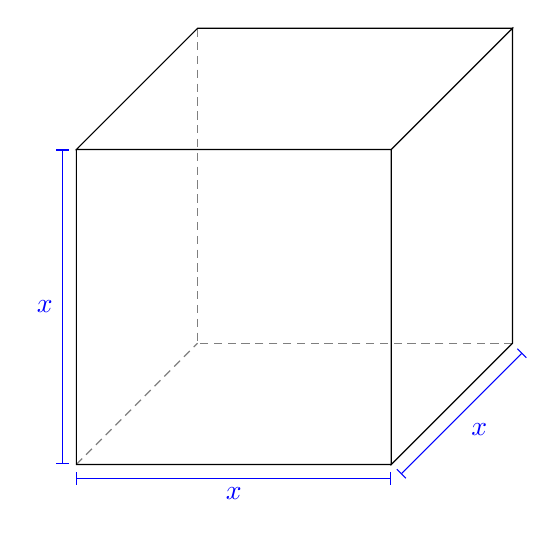
\begin{tikzpicture}[every edge quotes/.append style={auto, text=blue}]
      \pgfmathsetmacro{\cubex}{4}
      \pgfmathsetmacro{\cubey}{4}
      \pgfmathsetmacro{\cubez}{4}
      \draw[every edge/.append style={densely dashed, opacity=.5}]
      (0,0,0) coordinate (o) -- ++(-\cubex,0,0) coordinate (a) -- ++(0,-\cubey,0) coordinate (b) edge coordinate [pos=1] (g) ++(0,0,-\cubez)  -- ++(\cubex,0,0) coordinate (c) -- cycle (o) -- ++(0,0,-\cubez) coordinate (d) -- ++(0,-\cubey,0) coordinate (e) edge (g) -- (c) -- cycle (o) -- (a) -- ++(0,0,-\cubez) coordinate (f) edge (g) -- (d) -- cycle;
      \path [every edge/.append style={draw=blue, |-|}]
      (b) +(0,-5pt) coordinate (b1) edge ["$x$"'] (b1 -| c)
      (b) +(-5pt,0) coordinate (b2) edge ["$x$"] (b2 |- a)
      (c) +(3.5pt,-3.5pt) coordinate (c2) edge ["$x$"'] ([xshift=3.5pt,yshift=-3.5pt]e);
    \end{tikzpicture}
  \end{figure}
\end{frame}

\begin{frame}
  \begin{figure}[H]
    \centering
    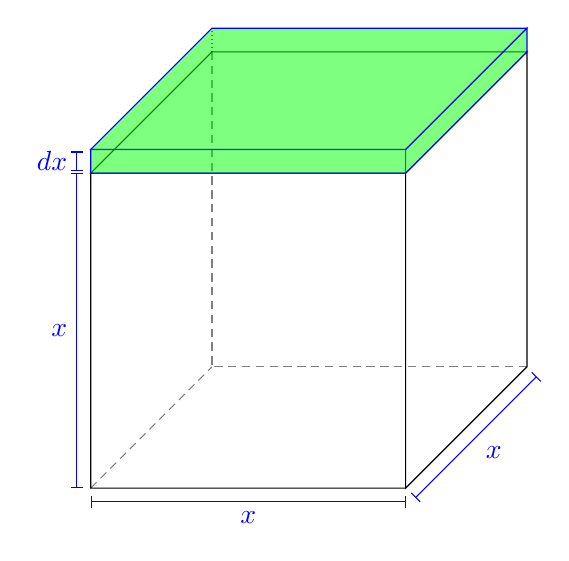
\begin{tikzpicture}[every edge quotes/.append style={auto, text=blue}]
      \pgfmathsetmacro{\cubex}{4}
      \pgfmathsetmacro{\cubey}{4}
      \pgfmathsetmacro{\cubez}{4}
      \pgfmathsetmacro{\dx}{.3}

      \draw[every edge/.append style={densely dashed, opacity=.5}]
      (0,0,0) coordinate (o) % node {o}
      -- ++(-\cubex,0,0) coordinate (a) % node {a}
      -- ++(0,-\cubey,0) coordinate (b) % node {b}
      edge coordinate [pos=1] (g) ++(0,0,-\cubez)
      -- ++(\cubex,0,0) coordinate (c) % node {c}
      -- cycle (o)
      -- ++(0,0,-\cubez) coordinate (d) % node {d}
      -- ++(0,-\cubey,0) coordinate (e) % node {e}
      edge (g)
      -- (c)
      -- cycle (o)
      -- (a)
      -- ++(0,0,-\cubez) coordinate (f) % node {f}
      edge (g) % node {g}
      -- (d)
      -- cycle;

      \coordinate (op) at (0,0,0);

      \draw[draw=blue, every edge/.append style={draw=blue, densely dashed, opacity=.5}, fill=green, fill opacity=.5]
      (op)
      -- ++(0,\dx,0) coordinate (h)
      -- ++(-\cubex, 0, 0) coordinate (i)
      -- ++(0,0,-\cubez) coordinate (j)
      -- ++(\cubex, 0, 0) coordinate (k)
      -- (h) -- cycle;

      \draw[draw=blue, every edge/.append style={draw=none}, fill=green, fill opacity=.5]
      (i)
      -- ++(0,-\dx, 0) coordinate (ip) edge coordinate [pos=1] (jp) ++(0,0,-\cubex) -- ++(\cubex, 0, 0) -- ++(0,0,-\cubez) -- ++(0,\dx,0) -- ++(0,0,\cubex);

      \draw[every edge/.append style={draw=blue, densely dotted, opacity=.5}]
      (jp) edge ++(0,\dx,0);

      \path [every edge/.append style={draw=blue, |-|}]
      (b) +(0,-5pt) coordinate (b1) edge ["$x$"'] (b1 -| c)
      (b) +(-5pt,0) coordinate (b2) edge ["$x$"] (b2 |- a)
      (c) +(3.5pt,-3.5pt) coordinate (c2) edge ["$x$"'] ([xshift=3.5pt,yshift=-3.5pt]e);
      \path [every edge/.append style={draw=blue, |-|}]
      (i) +(-5pt,-.025) coordinate (i1) edge ["$dx$"'] ++(-5pt,-.275)% (i1 -| a)
      ;
    \end{tikzpicture}
    \caption{Extending one side by $dx$}
  \end{figure}
\end{frame}
\begin{frame}
  \begin{figure}[H]
    \centering
    \includegraphics[keepaspectratio,width=.5\linewidth]{3b1b.png}
    \caption{3blue1brown's visualization (\cite{3b1b})}
  \end{figure}
\end{frame}
\begin{frame}{A final quote}{}
  \vfill\vspace{2em}
  \begin{aquote}{Marie-Sophie Germain}
    Algebra is but written geometry, and geometry is but figured algebra.
  \end{aquote}
  \vfill
\end{frame}


\section{Bibliography}
\begin{frame}
  \frametitle{References}
  \bibliographystyle{alpha}
  \bibliography{aha.bib}
\end{frame}

\end{document}


%%% Local Variables:
%%% mode: latex
%%% TeX-master: t
%%% End